\section{Experiments}

\subsection{Implementation Details}
\label{sec:exp:impl}
% 通用：
%   - Backbone：DINOv3 ViT-B（frozen）；T=8，224×224，ImageNet 归一化。
%   - 优化器：AdamW，weight decay 0.05，cosine schedule + 5-epoch warmup。
%   - 精度：bf16 autocast；grad accum=4，batch size 12（effective 48）。
%   - 正则：label smoothing 0.1，Mixup + CutMix，EMA decay=0.999。
%
% DINO-SPR：
%   - 可训练：LoRA r=8 + SSTS + KPTF + head；backbone 冻结，epochs 80。
%
% DINO-SPR Lite：
%   - Teacher frozen + bf16 detach；student 轻量 backbone + 共享 KPTF。
%   - 蒸馏 loss 权重见 §3.4；epochs 100。
%
% 硬件：单卡 RTX 4090（24GB），PyTorch 2.6，CUDA 12.4。

We adopt DINOv3 ViT-B as the default backbone with $T{=}8$ clips at $224{\times}224$.
Each frame is split into $N{=}196$ patch tokens of dimension $D{=}768$, and the
budget of the SSTS selection term is set to $K{=}0.3N$.
All models use AdamW (weight decay 0.05) with cosine schedule and 5-epoch warmup, 
gradient accumulation of 4 at batch size 12, label smoothing 0.1,
Mixup and CutMix, and EMA (decay 0.999).
For DINO-SPR, we keep the backbone largely frozen, training only LoRA adapters of
the last layer, SSTS, KPTF, and the linear
classification head for 80 epochs (lr $5{\times}10^{-4}$).
For DINO-SPR Lite, the frozen DINO-SPR teacher supervises a lightweight student,
trained for 100 epochs.
All training runs on a single RTX 4090 (24\,GB) with PyTorch 2.6 and CUDA 12.4.


% Dataset statistics table for TMI submission
\begin{table}[t]
\centering
\caption{Summary of the five surgical phase recognition datasets used in this study.}
\label{tab:datasets}
\setlength{\tabcolsep}{4pt}
\footnotesize
\begin{tabular}{lcccccc}
\toprule
\textbf{Dataset} & \textbf{Abbrev.} & \textbf{Country} & \textbf{\#Videos} & \textbf{\#Phases} & \textbf{Duration} \\
 & & & (train/val/test) & & \\
\midrule
Cholec80 & C80 & France & 32/8/40 & 7 & 51.3\,h \\
M2CAI16 & M16 & France & 22/5/14 & 8 & 26.3\,h \\
Cataract101 & Cat101 & Germany & 60/15/26 & 10 & 14.0\,h \\
CatPriv16 & CP16 & China & 25/5/11 & 16 & 10.0\,h \\
PitVis & PV & UK & 19/5/5 & 14 & 32.1\,h \\
\bottomrule
\end{tabular}
\end{table}

% 6-shot comparison table (private dataset)
\begin{table}[b]
\centering
\caption{Comparison of methods on 6-shot surgical phase recognition on our private CatPriv16 dataset.}
\label{tab:6shot_private}
\setlength{\tabcolsep}{4.0pt}
\footnotesize
\begin{tabular}{@{}l|ccccc@{}}
\toprule
\textbf{Method} & \textbf{Accuracy} & \textbf{Precision} & \textbf{Recall} & \textbf{F1} & \textbf{Jaccard} \\
\midrule
Trans-SVNet        & 68.2$\pm$0.4 & 55.3$\pm$1.0 & 45.1$\pm$1.7 & 45.0$\pm$1.0 & 35.9$\pm$0.9 \\
TeCNO              & 56.4$\pm$2.0 & 39.8$\pm$3.1 & 36.8$\pm$3.7 & 32.5$\pm$3.1 & 25.7$\pm$2.7 \\
MGTR-Net           & 70.3$\pm$0.7 & 54.2$\pm$1.2 & 50.8$\pm$0.7 & 48.6$\pm$0.8 & 40.5$\pm$0.7 \\
TMRNet             & 70.4$\pm$0.6 & 54.5$\pm$0.8 & 50.6$\pm$0.5 & 48.6$\pm$0.7 & 40.2$\pm$0.7 \\
Surgformer         & 66.3$\pm$0.4 & 49.4$\pm$0.1 & 44.7$\pm$1.4 & 43.1$\pm$1.2 & 35.5$\pm$1.0 \\
MuST               & 65.7$\pm$0.2 & 49.6$\pm$1.4 & 43.5$\pm$0.2 & 42.1$\pm$0.4 & 32.9$\pm$0.3 \\
LoViT$^\dagger$    & 59.2$\pm$2.0 & 36.5$\pm$0.4 & 35.7$\pm$0.4 & 31.6$\pm$0.4 & 24.0$\pm$0.3 \\
SKiT$^\dagger$     & 62.4$\pm$0.8 & 36.5$\pm$0.7 & 36.8$\pm$1.0 & 33.2$\pm$0.1 & 26.2$\pm$0.2 \\
\midrule
DINO-SPR           & \textbf{74.5$\pm$0.2} & \textbf{71.8$\pm$1.9} & \textbf{60.1$\pm$1.2} & \textbf{58.9$\pm$0.7} & \textbf{49.9$\pm$0.3} \\
\bottomrule
\end{tabular}

\vspace{6pt}
\begin{spacing}{0.95}
\end{spacing}
\end{table}

% 6-shot comparison table (four public datasets)
% 数据列保持 dataset-major（每个数据集下依次 Accuracy/Precision/Recall/F1/Jaccard）。
% 布局：上下两块已合并为一张 tabular，metrics 表头只在最顶部出现一次；
%   数据集名不单独占行，而是旋转 90° 竖排在该数据集数值区的左侧，
%   用 \multirow{9} 跨越各自 9 行数据行（Cholec80/Cataract101 覆盖 1-9 行，
%   M2CAI16/PitVis 覆盖 10-18 行，两块之间以 \midrule 分隔）。
\begin{table*}[t]
\centering
\caption{Comparison of methods on 6-shot surgical phase recognition across four public datasets. Best results are in \textbf{bold}. Results report mean$\pm$std across three independent runs under unrelaxed evaluation.}
\label{tab:6shot_public}
\setlength{\tabcolsep}{2.25pt}
\footnotesize

\begin{tabular}{@{}l|l|cccccc|cccccc@{}}
\toprule
\textbf{Method} & \textbf{Paradigm} & & \textbf{Accuracy} & \textbf{Precision} & \textbf{Recall} & \textbf{F1} & \textbf{Jaccard} & & \textbf{Accuracy} & \textbf{Precision} & \textbf{Recall} & \textbf{F1} & \textbf{Jaccard} \\
\midrule
Trans-SVNet & Multi-stage & \multirow{9}{*}{\rotatebox[origin=c]{90}{\textbf{Cholec80}}} & 72.8$\pm$0.5 & 62.8$\pm$1.9 & 61.2$\pm$0.4 & 55.9$\pm$1.0 & 43.4$\pm$0.9 & \multirow{9}{*}{\rotatebox[origin=c]{90}{\textbf{Cataract101}}} & 74.8$\pm$1.5 & 72.3$\pm$1.2 & 70.3$\pm$1.6 & 67.1$\pm$1.6 & 55.4$\pm$2.0 \\
TeCNO & Multi-stage &  & 56.6$\pm$3.7 & 46.8$\pm$1.8 & 49.5$\pm$0.5 & 41.3$\pm$1.7 & 30.0$\pm$1.6 &  & 58.9$\pm$1.5 & 53.0$\pm$1.7 & 54.0$\pm$1.5 & 48.6$\pm$1.3 & 37.4$\pm$1.1 \\
MGTR-Net & Multi-stage &  & 73.2$\pm$0.4 & 65.9$\pm$0.6 & 64.6$\pm$0.6 & 59.3$\pm$0.6 & 46.7$\pm$0.6 &  & 73.3$\pm$0.4 & 73.6$\pm$0.6 & 70.8$\pm$0.5 & 66.8$\pm$0.4 & 56.4$\pm$0.5 \\
TMRNet & Multi-stage &  & 72.1$\pm$0.3 & 63.6$\pm$0.3 & 63.6$\pm$0.6 & 58.0$\pm$0.4 & 45.2$\pm$0.4 &  & 72.6$\pm$0.5 & 71.7$\pm$0.7 & 69.8$\pm$1.0 & 65.3$\pm$0.5 & 54.8$\pm$0.6 \\
Surgformer & End-to-end &  & 64.4$\pm$0.9 & 59.7$\pm$0.1 & 62.8$\pm$0.6 & 58.2$\pm$0.4 & 48.6$\pm$0.5 &  & 72.4$\pm$0.3 & 69.9$\pm$0.5 & 70.1$\pm$0.2 & 66.9$\pm$0.3 & 56.8$\pm$0.3 \\
MuST & Multi-stage &  & 70.3$\pm$0.5 & 60.2$\pm$0.8 & 64.1$\pm$0.8 & 57.0$\pm$0.9 & 43.5$\pm$0.8 &  & 70.2$\pm$0.5 & 66.8$\pm$0.5 & 68.3$\pm$0.5 & 63.6$\pm$0.4 & 50.7$\pm$0.5 \\
LoViT$^\dagger$ & Multi-stage &  & 61.7$\pm$0.2 & 47.3$\pm$3.4 & 51.0$\pm$2.5 & 43.3$\pm$2.8 & 31.4$\pm$1.8 &  & 34.1$\pm$8.4 & 55.4$\pm$5.6 & 32.3$\pm$7.0 & 28.5$\pm$7.4 & 19.8$\pm$5.7 \\
SKiT$^\dagger$ & Multi-stage &  & 63.3$\pm$1.2 & 47.3$\pm$4.8 & 48.9$\pm$3.2 & 42.7$\pm$2.6 & 31.4$\pm$1.9 &  & 39.2$\pm$8.4 & 59.4$\pm$5.7 & 35.8$\pm$8.4 & 33.5$\pm$9.0 & 24.0$\pm$7.2 \\
DINO-SPR (DINOv3 ViT-B) & End-to-end &  & \textbf{80.1$\pm$0.2} & \textbf{72.7$\pm$0.1} & \textbf{76.6$\pm$0.8} & \textbf{70.7$\pm$0.5} & \textbf{58.1$\pm$0.4} &  & \textbf{85.2$\pm$0.1} & \textbf{83.4$\pm$0.1} & \textbf{82.7$\pm$0.1} & \textbf{79.5$\pm$0.2} & \textbf{71.0$\pm$0.2} \\
\midrule
Trans-SVNet & Multi-stage & \multirow{9}{*}{\rotatebox[origin=c]{90}{\textbf{M2CAI16}}} & 45.3$\pm$3.7 & 30.6$\pm$3.4 & 32.5$\pm$2.7 & 27.6$\pm$3.4 & 20.9$\pm$2.5 & \multirow{9}{*}{\rotatebox[origin=c]{90}{\textbf{PitVis}}} & 58.7$\pm$0.8 & 42.2$\pm$2.2 & 38.7$\pm$0.6 & 35.9$\pm$0.8 & 26.8$\pm$0.6 \\
TeCNO & Multi-stage &  & 31.1$\pm$3.4 & 26.3$\pm$1.8 & 26.5$\pm$0.3 & 22.2$\pm$0.7 & 14.4$\pm$0.6 &  & 44.6$\pm$2.9 & 29.0$\pm$1.3 & 27.7$\pm$3.4 & 24.7$\pm$1.9 & 17.7$\pm$1.5 \\
MGTR-Net & Multi-stage &  & 44.4$\pm$1.8 & 44.5$\pm$1.0 & 44.3$\pm$0.6 & 38.9$\pm$0.4 & 30.1$\pm$0.2 &  & 56.7$\pm$0.2 & 40.6$\pm$0.8 & 41.9$\pm$0.2 & 36.6$\pm$0.1 & 27.2$\pm$0.1 \\
TMRNet & Multi-stage &  & 38.3$\pm$4.8 & 37.3$\pm$0.4 & 38.8$\pm$2.9 & 32.3$\pm$2.4 & 23.8$\pm$1.5 &  & 55.3$\pm$1.3 & 38.5$\pm$1.5 & 40.4$\pm$0.7 & 34.3$\pm$0.9 & 24.9$\pm$0.8 \\
Surgformer & End-to-end &  & 61.6$\pm$0.5 & 55.3$\pm$0.5 & 59.9$\pm$0.7 & 54.0$\pm$0.6 & 44.8$\pm$0.8 &  & 52.1$\pm$0.7 & 40.4$\pm$0.7 & 38.0$\pm$0.5 & 35.8$\pm$0.6 & 27.1$\pm$0.5 \\
MuST & Multi-stage &  & 39.0$\pm$0.3 & 30.5$\pm$1.0 & 34.5$\pm$0.2 & 27.0$\pm$0.5 & 18.5$\pm$0.3 &  & 53.5$\pm$0.4 & 40.0$\pm$1.3 & 37.9$\pm$0.4 & 33.7$\pm$0.3 & 24.2$\pm$0.3 \\
LoViT$^\dagger$ & Multi-stage &  & 28.0$\pm$8.9 & 15.7$\pm$2.6 & 17.2$\pm$1.5 & 12.2$\pm$2.0 & 7.6$\pm$1.5 &  & 47.5$\pm$5.0 & 26.1$\pm$4.6 & 24.3$\pm$2.6 & 20.7$\pm$3.8 & 15.0$\pm$3.1 \\
SKiT$^\dagger$ & Multi-stage &  & 13.9$\pm$4.0 & 13.9$\pm$4.3 & 17.9$\pm$1.3 & 9.2$\pm$3.4 & 5.3$\pm$2.0 &  & 47.8$\pm$6.0 & 24.5$\pm$5.4 & 24.4$\pm$2.9 & 20.8$\pm$4.2 & 14.5$\pm$3.3 \\
DINO-SPR (DINOv3 ViT-B) & End-to-end &  & \textbf{72.3$\pm$0.8} & \textbf{64.9$\pm$1.1} & \textbf{71.5$\pm$0.5} & \textbf{62.9$\pm$0.2} & \textbf{50.6$\pm$0.3} &  & \textbf{67.9$\pm$1.1} & \textbf{59.1$\pm$1.0} & \textbf{53.8$\pm$0.6} & \textbf{52.9$\pm$0.3} & \textbf{41.3$\pm$0.3} \\
\bottomrule
\end{tabular}

\vspace{6pt}
\begin{spacing}{0.95}
\footnotesize
$^\dagger$LoViT and SKiT borrow the fine-tuned ResNet50 backbone from Trans-SVNet, as their original feature extractors are not publicly available.
\end{spacing}
\end{table*}



\begin{figure*}[t]
    \centering
    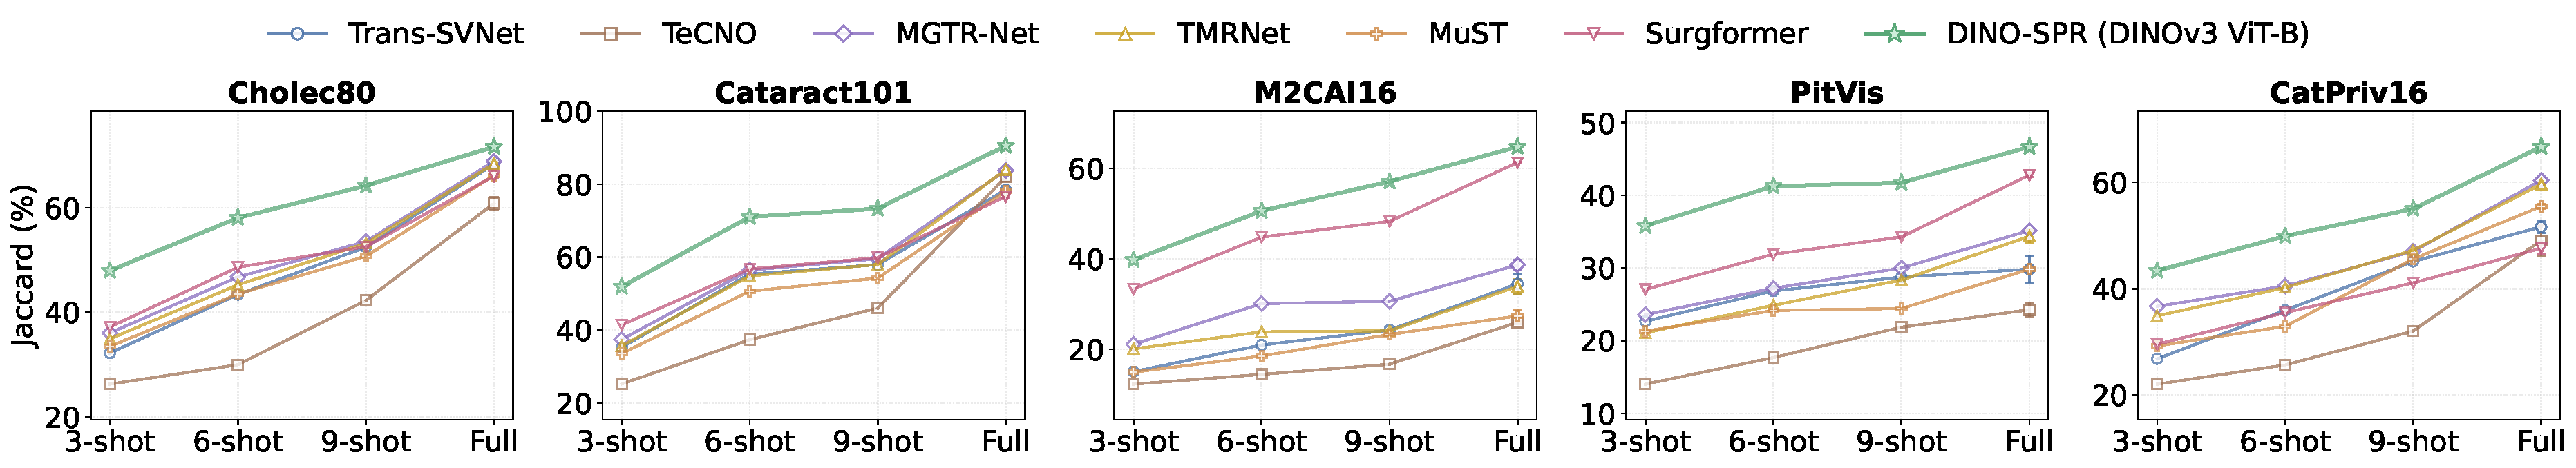
\includegraphics[width=\textwidth]{resources/fig_all_few_shot_trends_full.pdf}
    \caption{Few-shot trends (3-/6-/9-shot) of SPR-Teacher and prior methods on Jaccard, averaged over five datasets.}
    \label{fig:few-shot}
\end{figure*}

\subsection{Evaluation}
\subsubsection{Datasets}
% 5个数据集，覆盖3种手术类型（腹腔镜/眼科/神经外科），公开+私有联合评估。
% 对照 tab_dataset_description 过一遍关键数字即可，不做逐个介绍。
% 要点：(1) 公开数据集(Cholec80/M2CAI16/Cataract101/PitVis)作为行业标准baseline；
%       (2) 私有数据集(CatPriv16)评估跨中心泛化，无数据泄漏风险；
%       (3) 所有视频采样至1fps，few-shot split用3/6/9个标注视频。

To evaluate across diverse surgical scenarios, we curate five SPR
datasets spanning three procedure types: laparoscopic cholecystectomy (Cholec80,
M2CAI16), cataract surgery (Cataract101, CatPriv16), and transsphenoidal pituitary
surgery (PitVis), as summarized in Table~\ref{tab:datasets}. Among them,
CatPriv16 is our private dataset providing a
fully unseen reference for surgical FMs. All videos are sampled at
1\,fps, and few-shot splits use 3, 6, or 9 labeled training videos with unchanged
validation and test sets.

\subsubsection{Metrics}
% 一、SPR 主指标（unrelaxed evaluation）：
%   - 严格逐帧评估（unrelaxed / strict frame-by-frame），不做 temporal smoothing。
%   - 5个 macro-averaged metrics：Accuracy, Precision, Recall, F1, Jaccard。
%   - 均报告 mean±std over 3 seeds。
%   - 首推 Jaccard 作为主指标（最严格、最全面反映帧级分类质量）。
%
% 二、跨数据集一致性：
%   - mean Jaccard：多数据集平均，↑ 越高越好。
%   - Δ = max − min：跨数据集波动，↓ 越低表示泛化越均衡。
%
% 三、效率指标（对照 tab:efficiency，整表 CPU 单核口径）：
%   - Params (M)：部署网络总参数量，↓ 越低越好。
%   - GFLOPs：每帧计算量（backbone only，temporal overhead <0.1G），↓ 越低越好。
%   - FPS：forward-only 吞吐量，fp32、T=8 clip、单核 AMD EPYC 7543，↑ 越高越好。

Following prior work~\cite{jin2021temporal,yang2024surgformer}, we report accuracy,
precision, recall, F1-score, and Jaccard under unrelaxed evaluation, averaged over
three random seeds. We prioritize Jaccard for jointly penalizing frame-level false
positives and negatives, and summarize cross-dataset results by the mean Jaccard
together with the range $\Delta=\max-\min$, where a smaller $\Delta$ indicates more
balanced generalization. For deployment efficiency, we additionally report the
parameter count, per-frame GFLOPs, and the FPS of a single $T{=}8$ clip measured
on a single core of an AMD EPYC 7543 CPU.


\subsection{Comparisons with SOTAs}
\subsubsection{Few-shot Settings}
% 对照 tab_sota_6shot + fig_few_shot_trends：
%
% 1. SOTA 概览：
%   - 现有方法分两类：multi-stage（Trans-SVNet/MGTR-Net/TMRNet/MuST，ResNet50+时序）
%     和 end-to-end（Surgformer，3D ViT+HTA）。
%   - 6-shot 下 prior 方法 Jaccard 最高仅 56.8（Surgformer 在 Cat101），且跨数据集波动大。
%   - Multi-stage 方法依赖分步特征提取（数据量稀缺场景下无法充分微调特征提取器就会导致效果不佳，end-to-end Surgformer 精度尚可但极慢，CPU 单核仅 2.7 FPS）。
%
% 2. DINO-SPR 6-shot 表现（tab_sota_6shot）： ref这个 \label{tab:6shot}
%   - 5 数据集全部指标全面领先，Jaccard 相对最强 prior 高 5.8-14.2 点。
%   - 举具体例子：Cholec80 58.1 vs best SOTA 48.6，Cataract101 71.0 vs 56.8，
%     CatPriv16 49.9 vs 40.5，M2CAI16 50.6 vs 44.8。
%   - 单遍端到端 vs SOTA 两阶段，计算效率对比见 §comp cost。
%
% 3. Few-shot trend（fig_few_shot_trends）： ref这个 \label{fig:few-shot}
%   - 3/6/9-shot 全区间一致领先，DINO-SPR 6-shot 已超 SOTA 9-shot。
%   - 随 shot 数减少，SOTA 急剧下降（e.g. Trans-SVNet Cat101: 9-shot 42→3-shot 26），
%     DINO-SPR 下降平缓（78→55），体现 FM 先验对少样本的鲁棒性。
%   - 举 1-2 个数据集的 trend 例子。

We compare DINO-SPR with eight prior methods spanning two paradigms.
Multi-stage methods, namely Trans-SVNet~\cite{gao2021trans},
TeCNO~\cite{czempiel2020tecno}, MGTR-Net~\cite{huang2025multi},
TMRNet~\cite{jin2021temporal}, MuST~\cite{perez2024must}, LoViT~\cite{liu2025lovit},
and SKiT~\cite{liu2023skit}, fine-tune a backbone before appending a temporal
model. Surgformer~\cite{yang2024surgformer}, the only end-to-end approach, instead
jointly models multiple input frames through spatiotemporal attention in a ViT.
Tables~\ref{tab:6shot_public} and~\ref{tab:6shot_private} report the 6-shot
comparison over the four public datasets and our private CatPriv16, respectively.

Under few-shot supervision, multi-stage methods generally lag behind, since scarce
labels do not allow their feature extractors to be fine-tuned well, whereas the
end-to-end Surgformer performs somewhat better. Leveraging the strong pretraining of
DINOv3 and our few-shot specific spatiotemporal adaptation, DINO-SPR clearly
surpasses all prior methods on every metric and dataset, reaching 58.1, 71.0, and
49.9 Jaccard on Cholec80, Cataract101, and CatPriv16. These scores improve on the
strongest prior method by 9.5, 14.2, and 9.4 on each dataset, and the gains span
5.8 to 14.2 across the five datasets. Figure~\ref{fig:few-shot} further shows that
DINO-SPR leads by a large margin at every label budget. 
The advantage is largest at the extreme 3-shot setting, for instance on M2CAI16,
where DINO-SPR reaches 39.7 Jaccard while the prior method TeCNO falls to
12.3, demonstrating that our method fully exploits the potential of foundation
models.


% VFM backbone-selection ablation (backbone comparison figure)
\begin{figure*}[!hb]
    \centering
    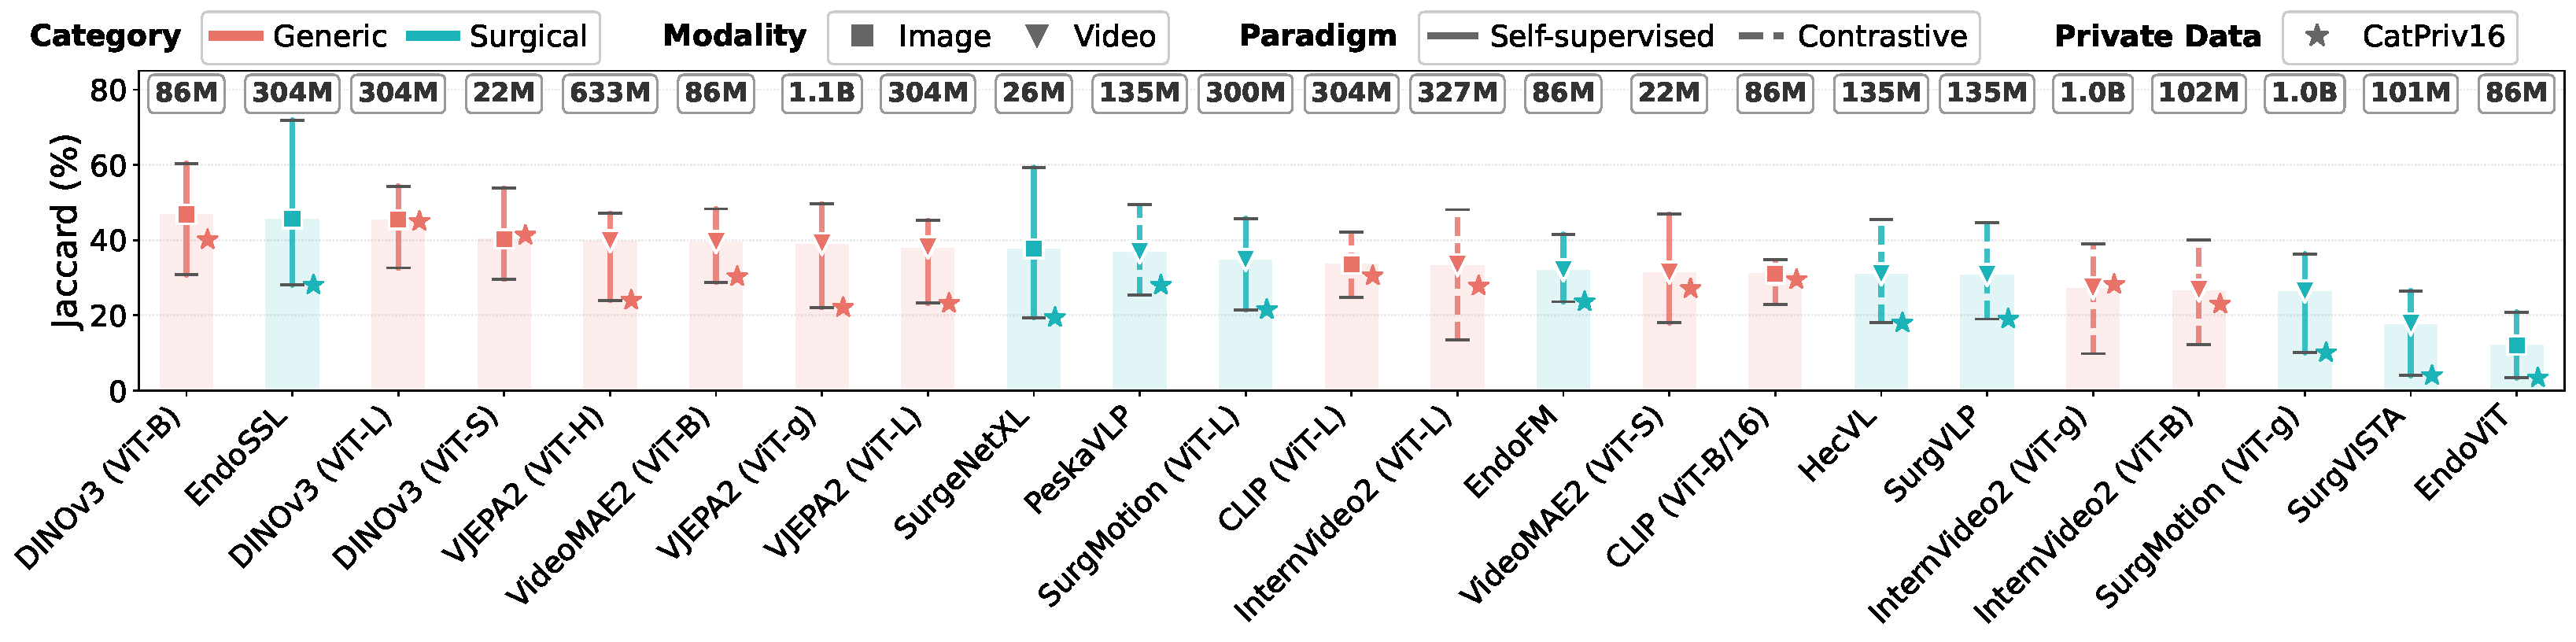
\includegraphics[width=\textwidth]{resources/fig_vfm_backbone.pdf}
    \caption{Ablation of foundation models as the frozen backbone under 6-shot surgical phase recognition with MGTR-Net as the temporal model. For each foundation model, sorted by decreasing mean Jaccard, the vertical bar spans the min--max Jaccard across the five datasets, and the shape marker marks the mean Jaccard. The star marks the private CatPriv16 dataset as an unseen domain, and the labeled value is the parameter size.}
    \label{fig:vfm_backbone}
\end{figure*}



\subsubsection{Computational Cost and Parameter Efficiency}
% 对照 tab_efficiency（整表已改为 CPU 单核口径）：
%
% 1. SOTA 效率问题：
%   - Multi-stage 方法：两遍推理（ResNet50 逐帧提特征 → 时序模型），无法流式处理；
%     ResNet50 前端本身就卡死在 ~8 FPS（Trans-SVNet 8.3 / MGTR-Net 8.2 / MuST 8.4）。
%   - Surgformer：端到端但 121M ViT，CPU 上最慢，仅 2.7 FPS。
%   - SOTA 准确率低（43-49 J）且效率差，难以实际部署。
%
% 2. DINO-SPR：精度最高（58.1 J），但同为 ViT，CPU 上 2.6 FPS、不比 Surgformer 快
%   → 由此引出「精度高 ≠ 可部署」这个动机，再转入蒸馏。
%
% 3. DINO-SPR Lite：异构蒸馏，按目标硬件挑 backbone。
%   - 关键结论：过 25 FPS 线的两个都是 CNN（ConvNeXt-Atto 43.7、StarNet-S4 26.0），
%     而同量级的 ViT 学生 TinyViT-5M 只有 18.6 —— 速度不自动跟着尺寸走。
%   - 待办：图 fig_computational_cost 仍是 GPU/Cataract101 口径，与本节的 CPU 口径不一致。

Clinical deployment often has to work without a dedicated GPU, so we emulate such a
limited environment by measuring all inference on a single CPU core, as reported in
Table~\ref{tab:efficiency} for 6-shot Cholec80.
Prior methods were not designed for real-time inference, and their FPS
only spans 2.7 to 8.4, far below the 25\,FPS native video rate.
Surgformer is the slowest because it jointly attends over all frames of a clip with
a 121M ViT.
DINO-SPR reaches 58.1 Jaccard, yet as a ViT it inherits the same limit
and runs at 2.6\,FPS.
High performance alone thus does not make a model deployable.
Architecture-agnostic distilling DINO-SPR into lightweight students closes that gap and meets the real-time requirement, reaching up to
44\,FPS on a single CPU with performance close to DINO-SPR.

% Efficiency comparison — measured on a single CPU core (AMD EPYC 7543).
% Forward-only, fp32, T=8 clip, batch 1, fps = T / (clip_latency_s),
% median over rounds; raw clip_ms in latex/resources/:
%   cpu_throughput_deployed.json  (Lite rows: deployed DistillStudent, 7x30)
%   cpu_throughput_sota.json      (two-stage rows: ResNet50 + temporal, 5x20)
%   cpu_throughput_final.json     (Surgformer / DINOv3 ViT-B surrogates)
% Params are whole-model counts (backbone + temporal + head) for the Lite rows
% and for Trans-SVNet (25.1M) / MGTR-Net (46.6M).  MuST is the exception: its
% 68.0M is the reported four-stage pipeline (MViT + MTFE + TCM), whereas the
% FPS comes from the ResNet50 surrogate actually timed here (37.2M).
% GFLOPs count the backbone only (temporal overhead <0.1 G).
% Full-node (64-thread) runs excluded: external load on the shared node made
% small-model values swing 2-256 fps.
% The two-stage rows are two-pass pipelines (ResNet50 features precomputed for
% the whole video), so their FPS is a compute rate, not a streaming rate.
\begin{table}[t]
\centering
\caption{Computational cost and performance on 6-shot Cholec80.}
\label{tab:efficiency}
\setlength{\tabcolsep}{3.0pt}
\footnotesize
\begin{tabular}{@{}l@{\hspace{2pt}}r r r r@{}}
\toprule
\textbf{Method} & \textbf{Params}$\downarrow$ & \textbf{GFLOPs}$\downarrow$ & \textbf{FPS}$\uparrow$ & \textbf{Jaccard}$\uparrow$ \\
\midrule
\multicolumn{5}{l}{\textbf{Prior SOTA}} \\
\quad Trans-SVNet        & 25.1M  & 4.1  & 8.3  & 43.4 \\
\quad MGTR-Net           & 46.6M  & 4.1  & 8.2  & 46.7 \\
\quad MuST               & 68.0M  & 10.6 & 8.4  & 43.5 \\
\quad Surgformer         & 121.3M & 22.5 & 2.7  & 48.6 \\
\midrule
\multicolumn{5}{l}{\textbf{DINO-SPR}} \\
\quad DINOv3 ViT-B       & 92.0M  & 17.6 & 2.6  & 58.1 \\
\midrule
\multicolumn{5}{l}{\textbf{DINO-SPR Lite}} \\
\quad TinyViT-5M         & 7.1M & 1.2  & 18.6 & 55.4 \\
\quad StarNet-S4         & 8.9M & 1.1  & 26.0 & 55.2 \\
\quad ConvNeXt-Atto      & 5.4M & 0.6  & 43.7 & 52.2 \\
\bottomrule
\end{tabular}
\end{table}




\subsection{Ablation Study}
\subsubsection{Foundation Model Selection}
% 目的：把 FM benchmark 降级为 backbone 选择的 ablation。两段：config + 图要点。
% 实验设定：冻住各 FM 提特征，MGTR-Net 作时序，6-shot 5 数据集，隔离 FM 特征迁移性。
% 图要点：mean/range/CatPriv16/params；通用 FM 优于手术 FM；DINOv3 是最优起点。

To investigate how FMs generalize to few-shot SPR, we freeze each FM as a
feature extractor and train MGTR-Net~\cite{huang2025multi} as the temporal model on
8-frame windows, under the unified 6-shot protocol across five datasets.
Since surgical FMs may have seen the evaluation datasets during pretraining, we
highlight our private CatPriv16 as a leakage-free reference for fair generalization.

Figure~\ref{fig:vfm_backbone} ranks all FMs by mean Jaccard.
General FMs achieve higher Jaccard with more stable cross-dataset
generalization than surgical FMs.
The instability of surgical FMs likely stems from their pretraining data covering
certain procedure types more thoroughly. On the leakage-free CatPriv16, surgical FMs
nearly all rank at their worst, suggesting their true generalization is weaker than
their inflated scores imply.
By pretraining paradigm, SSL methods outperform contrastive ones, as SSL steers the
model toward spatial details while the contrastive objective is more global and thus
less suited to the spatially discriminative nature of SPR.
Video input does not clearly surpass image input, while incurring a larger
computational burden and parameter count. For instance, VideoMAE2 ViT-g with 1B parameters reaches
47.2, only marginally above the 86M DINOv3 ViT-B at 46.9.
We therefore adopt DINOv3~\cite{simeoni2025dinov3} as the backbone, as it exhibits
strong generalization despite having seen almost no surgical data during pretraining.

% VFM configuration summary (single-column, one row per method)
\begin{table}[t]
\centering
\caption{Configurations of the compared foundation models.}
\label{tab:vfm_config}
\setlength{\tabcolsep}{1.2pt}
\footnotesize
\begin{tabular}{@{}l@{\hspace{12pt}}llll@{}}
\toprule
\multicolumn{1}{l}{\textbf{Method}} & \multicolumn{1}{c}{\textbf{Backbone}} & \multicolumn{1}{c}{\textbf{Paradigm}} & \multicolumn{1}{c}{\textbf{Modality}} & \multicolumn{1}{c}{\textbf{Data}} \\
\midrule
\multicolumn{5}{@{}l}{\textbf{General FMs}} \\
DINOv3 & ViT & DINO & I & 1.7B images \\
CLIP & ViT & CTR & I+T & 400M images \\
VideoMAE2 & ViT & MAE & V & 1.35M videos \\
VJEPA2 & ViT & JEPA & V & 2M videos \\
InternVideo2 & ViT & MAE+CTR & V+T & 1.1M videos \\
\midrule
\multicolumn{5}{@{}l}{\textbf{Surgical FMs}} \\
EndoSSL & ViT & MSN & I & 23.3M images \\
SurgeNetXL & CAFormer & DINO & I & 4.7M images \\
EndoViT & ViT & MAE & I & 744K images \\
SurgMotion & ViT & JEPA & V & 15M videos \\
EndoFM & ViT & MAE & V & 33K videos \\
SurgVISTA & ViT & MAE & V & 3.7K videos \\
PeskaVLP & ResNet+BERT & CTR & V+T & 1.3K videos \\
HecVL & ResNet+BERT & CTR & V+T & 1.3K videos \\
SurgVLP & ResNet+BERT & CTR & V+T & 1.3K videos \\
\bottomrule
\end{tabular}
\vspace{3pt}
\begin{spacing}{0.95}
\footnotesize
I/V/T denotes image/video/text. MAE, DINO, JEPA, and MSN belong to self-supervised learning, while CTR is contrastive learning.
\end{spacing}
\end{table}



\subsubsection{DINOv3 Pretraining and Scale}
% 对照 tab_dinov3_finetune：
%   - 同 ViT-B 架构下对比 Random / IN-1K / DINOv3 三种预训练权重 + Frozen / Finetune 两种模式。
%   - DINOv3 + Finetune 在所有 shot 下均为最优，显著优于 IN-1K + Finetune。
%   - 跨规模对比：ViT-S/B/L，ViT-B 在效果与效率之间最佳平衡，选为主干。
%   - Random 仅保留 Finetune 对照；其表现远落后预训练权重，说明预训练先验不可或缺。
To understand DINOv3's promising few-shot performance, we first probe
the backbone with single frames ($T{=}1$), before adding any temporal module.
Table~\ref{tab:dinov3_finetune} reports this ablation, from which three findings
emerge.
First, pretraining largely decides the outcome, with Jaccard climbing steadily from
random to ImageNet-1K to DINOv3 weights even when the features are frozen.
Fine-tuned DINOv3 ViT-B reaches 48.6 Jaccard on Cholec80 at 6-shot, versus 42.9 for
ImageNet-1K.
Second, scaling yields diminishing returns beyond ViT-B.
Moving from ViT-S to ViT-B brings clear gains, whereas ViT-L improves only marginally
at 3.5$\times$ the parameters (304M versus 86M).
Third, fine-tuning consistently outperforms frozen features.
These findings lead us to adopt DINOv3 ViT-B for its accuracy-efficiency balance and
to fine-tune it in all subsequent experiments.


% DINOv3 Fine-tune vs Frozen Ablation with Pretraining Controls --- Single Column
% T=1 (single frame), Jaccard only.
\begin{table}[t]
\centering
\caption{Backbone pretraining and fine-tuning ablation at T$=$1 (single frame).
We compare random, ImageNet-1K, and DINOv3 weights under frozen and fine-tuned modes across ViT sizes.}
\label{tab:dinov3_finetune}
\footnotesize
\setlength{\tabcolsep}{2.4pt}
\begin{tabular}{@{}l l|rrr|rrr@{}}
\toprule
\multirow{2}{*}{Weights} & \multirow{2}{*}{Mode} & \multicolumn{3}{c}{Cholec80} & \multicolumn{3}{c}{Cataract101} \\
\cmidrule(lr){3-5} \cmidrule(lr){6-8}
& & 3-shot & 6-shot & 9-shot & 3-shot & 6-shot & 9-shot \\
\midrule
\multicolumn{8}{l}{\textbf{ViT-S (22M)}} \\
\quad Random  & Finetune & 21.2 & 24.8 & 28.0 & 10.9 & 16.0 & 16.7 \\
\quad IN-1K    & Frozen   & 30.5 & 33.8 & 35.6 & 22.4 & 29.4 & 31.3 \\
\quad IN-1K    & Finetune & 37.8 & 42.9 & 51.7 & 40.2 & 55.8 & 58.4 \\
\quad DINOv3   & Frozen   & 33.0 & 37.2 & 39.7 & 26.8 & 33.7 & 35.5 \\
\quad DINOv3   & Finetune & \textbf{37.4} & \textbf{44.7} & \textbf{51.9} & \textbf{34.7} & \textbf{55.4} & \textbf{55.1} \\
% \quad DINOv3   & LoRA     & 39.7 & 46.9 & 53.4 & 42.5 & 55.5 & 57.7 \\
\midrule
\multicolumn{8}{l}{\textbf{ViT-B (86M)}} \\
\quad Random  & Finetune & 20.3 & 25.4 & 29.3 & 13.1 & 17.8 & 20.3 \\
\quad IN-1K    & Frozen   & 34.0 & 37.5 & 39.7 & 25.7 & 35.2 & 37.2 \\
\quad IN-1K    & Finetune & 37.0 & 42.9 & 50.1 & 42.2 & 57.2 & 58.7 \\
\quad DINOv3   & Frozen   & 35.6 & 38.8 & 42.3 & 26.1 & 34.6 & 35.3 \\
\quad DINOv3   & Finetune & \textbf{40.9} & \textbf{48.6} & \textbf{54.7} & \textbf{40.9} & \textbf{56.9} & \textbf{62.2} \\
% \quad DINOv3   & LoRA     & 39.1 & 47.8 & 54.7 & 42.9 & 57.1 & 60.2 \\
\midrule
\multicolumn{8}{l}{\textbf{ViT-L (304M)}} \\
\quad Random  & Finetune & 21.0 & 26.2 & 31.3 & 14.5 & 19.9 & 22.0 \\
\quad IN-1K    & Frozen   & 33.2 & 41.3 & 43.0 & 31.9 & 43.3 & 46.2 \\
\quad IN-1K    & Finetune & 37.2 & 44.4 & 49.4 & 45.9 & 56.5 & 56.7 \\
\quad DINOv3   & Frozen   & 36.2 & 42.0 & 45.0 & 26.2 & 35.0 & 36.4 \\
\quad DINOv3   & Finetune & \textbf{42.7} & \textbf{49.7} & \textbf{55.3} & \textbf{47.3} & \textbf{61.8} & \textbf{63.0} \\
% \quad DINOv3   & LoRA     & 44.1 & 48.7 & 57.6 & 46.2 & 60.0 & 60.4 \\
\bottomrule
\end{tabular}
\end{table}

% Spatiotemporal Design Ablation --- Single Column
% Control-variable, 3 progressive regions on DINOv3 ViT-B, 6-shot, Jaccard (J), 1 decimal.
% Gains vs. region baseline in parentheses. R1 baseline: Frozen DINOv3 (CLS).
% R2/R3 baseline: Frozen+LoRA+SSTS (best of R1).
\begin{table}[!ht]
\centering
\caption{Spatiotemporal design ablation on 6-shot training.}
\label{tab:temporal_modeling}
\small
\setlength{\tabcolsep}{3pt}
\begin{tabular}{l c c c}
\toprule
Method & T & Cataract101 & Cholec80 \\
\midrule
\multicolumn{4}{l}{\textbf{R1. Single frame (T=1): spatial design}} \\
\quad Frozen DINOv3 (CLS)              & 1  & 34.6            & 38.8 \\
\quad Fine-tuned DINOv3 (full)       & 1  & 55.0 {\scriptsize (+20.4)} & 46.1 {\scriptsize (+7.3)} \\
\quad Frozen + LoRA (CLS)            & 1  & 55.2 {\scriptsize (+20.6)} & 45.5 {\scriptsize (+6.7)} \\
\quad Frozen + LoRA + mean-patch     & 1  & 53.0 {\scriptsize (+18.4)} & 45.8 {\scriptsize (+7.0)} \\
\quad Frozen + LoRA + SSTS (ours)    & 1  & \textbf{57.7 {\scriptsize (+23.1)}} & \textbf{49.6 {\scriptsize (+10.8)}} \\
\midrule
\multicolumn{4}{l}{\textbf{R2. Simple temporal fusion}} \\
\quad Frozen+LoRA+SSTS (T=1)          & 1  & 57.7            & 49.6 \\
\quad + Mean Pooling   & 4  & 57.8 {\scriptsize (+0.1)}  & 49.8 {\scriptsize (+0.2)} \\
\quad + Mean Pooling   & 8  & 58.2 {\scriptsize (+0.5)}  & 51.2 {\scriptsize (+1.6)} \\
\quad + Max Pooling    & 4  & 61.5 {\scriptsize (+3.8)}  & 49.0 {\scriptsize (-0.6)} \\
\quad + Max Pooling    & 8  & 62.8 {\scriptsize (+5.1)}  & 51.5 {\scriptsize (+1.9)} \\
\quad + Bi-LSTM        & 4  & 60.2 {\scriptsize (+2.5)}  & 52.0 {\scriptsize (+2.4)} \\
\quad + Bi-LSTM        & 8  & \textbf{65.0 {\scriptsize (+7.3)}}  & \textbf{53.5 {\scriptsize (+3.9)}} \\
\midrule
\multicolumn{4}{l}{\textbf{R3. Spatiotemporal fusion (ours)}} \\
\quad Frozen+LoRA+SSTS (T=1)          & 1  & 57.7            & 49.6 \\
\quad + KPTF           & 4  & 64.6 {\scriptsize (+6.9)}  & 53.9 {\scriptsize (+4.3)} \\
\quad + KPTF           & 8  & 71.0 {\scriptsize (+13.3)}  & \textbf{58.1 {\scriptsize (+8.5)}} \\
\quad + KPTF           & 16 & \textbf{76.1 {\scriptsize (+18.4)}}  & 57.3 {\scriptsize (+7.7)} \\
\bottomrule
\end{tabular}
\end{table}



\subsubsection{Different Spatiotemporal Modeling}
% 对照 tab_temporal_modeling：
%   - R1（单帧 T=1）：Frozen DINov3 CLS 仅 38.8/34.6；LoRA 微调涨至 45.5/55.2；
%     LoRA + SSTS 达到 49.6/57.7，验证 SSTS 空间注意力有效性。
%   - R2（简单时序融合）：增加 T 普遍带来增益；Mean/Max Pooling 过于 naive；
%     Bi-LSTM 简单有效，T=8 时涨至 53.5/65.0。
%   - R3（KPTF）：进一步涨至 58.1/71.0（T=8），T=8 为效率与效果平衡点。
Table~\ref{tab:temporal_modeling} ablates spatial and temporal design choices on
Cholec80 and Cataract101 at 6-shot, from single frames to full temporal fusion.
In R1, we freeze the DINOv3 backbone and fine-tune a linear classifier on its CLS
token, which yields only 38.8 and 34.6 Jaccard.
LoRA fine-tuning, which matches full fine-tuning at a fraction of the cost, lifts
Jaccard to 45.5 and 55.2, and our SSTS module further raises it to 49.6 and 57.7,
confirming the value of salient spatial token selection.
In R2, temporal fusion over this R1-best setup adds clear gains as the clip lengthens,
and a lightweight Bi-LSTM is the strongest simple aggregator, reaching 53.5 and 65.0
at T$=$8.
In R3, our KPTF module, which guides temporal fusion by keyframe priors, surpasses
Bi-LSTM at every clip length, reaching 58.1 and 71.0 at T$=$8.
Since longer clips do not necessarily bring further gains, we adopt T$=$8 as the
default.

% Distillation model comparison across three lightweight families, curated students.
% 6-shot, T=8, Jaccard (%). Each data cell: "w/o KD -> w/ KD" (student-only -> CAP + STGD).
% Arrow notation explained in caption; Family labels in region headers.
% Within each family, same-series models grouped together, sorted by parameter count.
% Params are DEPLOYED counts: backbone + student spatial attention + dim adapter +
%   temporal fusion + head (distill3mod stage B), i.e. what actually runs at
%   inference -- not the bare timm backbone.  Measured 2026-09-10; the teacher
%   row keeps its whole-model count.  Note: the MobileOne rows show the
%   training-time (un-reparameterized) form, which is much larger than the
%   fused inference form.
% Commented-out series (distilled accuracy trails same-family alternatives):
%   Pure CNN: MobileNetV3-Large, MobileOne-S1/S2; ViT-based: DeiT-Tiny/Small, RepViT-M1.1.
% 2026-09-05: student-only baselines lowered so a tiny student trained on 6-shot task
%   loss stays below the strongest prior (Surgformer) in each dataset, by -10 Jaccard on
%   Cataract101 and -3 on Cholec80. Distilled (w/ KD) values unchanged.
\begin{table}[b]
\centering
\caption{Distillation of SPR-Teacher into lightweight students on 6-shot settings.
Each cell: student-only $\rightarrow$ distilled.}
\label{tab:distill_models}
\small
\setlength{\tabcolsep}{4pt}
\begin{tabular}{l c c c}
\toprule
Model & Params$\downarrow$ & Cataract101$\uparrow$ & Cholec80$\uparrow$ \\
\midrule
\multicolumn{4}{l}{\textbf{Teacher}} \\
\quad SPR-Teacher (ViT-B)            & 92M  & 71.0            & 58.1 \\
\midrule
\multicolumn{4}{l}{\textbf{Pure CNN}} \\
\quad ConvNeXt-Atto               & 5.4M & 50.2 $\rightarrow$ 71.6 & 39.8 $\rightarrow$ 52.2 \\
\quad ConvNeXt-Tiny               & 33.3M & 53.6 $\rightarrow$ \textbf{72.2}          & 43.3 $\rightarrow$ \textbf{57.8} \\
\quad StarNet-S2                  & 5.1M & 51.3 $\rightarrow$ 69.7          & 36.6 $\rightarrow$ 52.3 \\
\quad StarNet-S4                  & 8.9M & 52.4 $\rightarrow$ 71.7          & 44.2 $\rightarrow$ 55.2 \\
\quad MobileNetV3-Small           & 3.6M & 50.2 $\rightarrow$ 66.8          & 43.1 $\rightarrow$ 53.0 \\
%\quad MobileNetV3-Large           & 7.1M & 37.2 $\rightarrow$ 61.0          & 34.2 $\rightarrow$ 52.3 \\
%\quad MobileOne-S1                & 9.3M & 46.7 $\rightarrow$ 64.9          & 33.6 $\rightarrow$ 52.4 \\
%\quad MobileOne-S2                & 17.4M & 48.1 $\rightarrow$ 69.1          & 34.3 $\rightarrow$ 52.9 \\
\midrule
\multicolumn{4}{l}{\textbf{ViT-based}} \\
\quad TinyViT-5M                  & 7.1M & 45.8 $\rightarrow$ 70.9          & 41.9 $\rightarrow$ 55.4 \\
\quad TinyViT-11M                 & 12.8M & 47.5 $\rightarrow$ \textbf{72.3}          & 45.0 $\rightarrow$ \textbf{57.5} \\
\quad RepViT-M0.9                 & 6.9M & 45.8 $\rightarrow$ 65.2          & 36.1 $\rightarrow$ 52.0 \\
%\quad RepViT-M1.1                 & 10.2M & 40.2 $\rightarrow$ 66.1          & 37.4 $\rightarrow$ 49.8 \\
%\quad DeiT-Tiny                   & 7.3M & 36.9 $\rightarrow$ 60.2          & 41.5 $\rightarrow$ 51.2 \\
%\quad DeiT-Small                  & 23.8M & 41.8 $\rightarrow$ 63.0          & 42.9 $\rightarrow$ 53.5 \\
\midrule
\multicolumn{4}{l}{\textbf{Hybrid}} \\
\quad MobileViTv2-100             & 6.8M & 47.0 $\rightarrow$ 66.2          & 43.3 $\rightarrow$ 55.4 \\
\quad MobileViTv2-150             & 13.1M & 43.0 $\rightarrow$ \textbf{71.0}          & 35.7 $\rightarrow$ \textbf{55.5} \\
\quad EdgeNeXt-XXS                & 2.9M & 45.6 $\rightarrow$ 67.9          & 37.6 $\rightarrow$ 53.3 \\
\quad EdgeNeXt-XS                 & 4.0M & 48.5 $\rightarrow$ 68.8          & 40.7 $\rightarrow$ 54.7 \\
\bottomrule
\end{tabular}
\end{table}


\subsubsection{Different Lightweight Models for DINO-SPR Lite}
% 对照 tab_distill_models：
%   - CNN / ViT / Hybrid 三类架构通过统一 CAP+STGD 蒸馏，student-only → distilled 均有显著增益。
%   - ConvNeXt-Atto（5.4M 部署口径）蒸馏后 Cat 达 71.6 J，超过 teacher。
%   - 异构蒸馏使部署端可自由选择最适合硬件的 backbone 族。
Table~\ref{tab:distill_models} compares each student trained from scratch and after
architecture-agnostic distillation on Cataract101 and Cholec80.
Distillation improves every mainstream lightweight backbone across the three
architecture categories, by over 20 Jaccard on average on Cataract101, confirming
that it transfers DINO-SPR knowledge to heterogeneous students.
In particular, the strongest student of each family reaches 72.2, 72.3, and 71.0 for
ConvNeXt-Tiny, TinyViT-11M, and MobileViTv2-150, respectively, matching or exceeding
the 92M teacher's 71.0 on Cataract101.
Distillation thus allows picking the backbone best suited to the deployment
setting with little performance loss.

% Distillation ablation, non-cumulative: each component trained alone and jointly.
% Aligned to the overall objective L = L_CE + L_cap + L_stgd (STGD bundles the
% representation, prior, and logit terms). One CNN student (ConvNeXt-Atto,
% heterogeneous, the design target of CAP); two dataset columns. The student-only
% baseline row is kept for reference. Same frozen SPR-Teacher teacher (dsx_bilstm).
% 6-shot, T=8, Jaccard (%). Gains vs. student-only in parentheses.
% src: research_logs/CAP_architecture_agnostic_distillation.md
% 2026-09-05: CE baseline matches the scaled ConvNeXt-Atto no-KD of tab_distill_models
%   (Cataract101 50.2 / Cholec80 39.8); last row = complete scheme = the distilled
%   ConvNeXt-Atto in tab_distill_models. The CAP-only and STGD-only values are
%   placeholders (not re-run); the last row holds the real values.
\begin{table}[t]
\centering
\caption{Distillation design ablation on 6-shot setting.}
\label{tab:distill_strategy}
\small
\setlength{\tabcolsep}{5pt}
\begin{tabular}{l c c}
\toprule
ConvNeXt-Atto (CNN) & Cataract101 & Cholec80 \\
\midrule
Student only (w/o distillation)                & 50.2                   & 39.8                   \\
+ $L_\mathrm{cap}$ (CAP only)                 & 62.4 {\scriptsize (+12.2)} & 47.0 {\scriptsize (+7.2)} \\
+ $L_\mathrm{stgd}$ (STGD only)               & 59.0 {\scriptsize (+8.8)} & 44.8 {\scriptsize (+5.0)} \\
+ $L_\mathrm{cap}$ + $L_\mathrm{stgd}$ (Full method) & 71.6 {\scriptsize (+21.4)} & 52.2 {\scriptsize (+12.4)} \\
\bottomrule
\end{tabular}
\end{table}



\subsubsection{Different Distillation Strategies}
% 对照 tab_distill_strategy（CNN 学生 ConvNeXt-Atto）：
%   - 非累积消融，行标签用 method 顶层 loss term：student-only($L_{CE}$) 参照行 +
%     单独 $L_{cap}$(CAP)、单独 $L_{stgd}$(STGD)、$L_{cap}$+$L_{stgd}$(完整)。
%   - baseline 与 tab_distill_models 的 Atto no-KD 对齐（50.2/39.8，已按 SOTA 下调）；末行=71.6/52.2。
%   - CAP/STGD 单独值为占位（未重跑），末行与 tab_distill_models 的 distilled 一致。
We ablate the distillation components on the heterogeneous CNN ConvNeXt-Atto in
Table~\ref{tab:distill_strategy}. Training with the task loss $L_\mathrm{CE}$ alone stays
weak at 50.2 on Cataract101, because the scarce labels offer little supervision
to the small model. Adding $L_\mathrm{cap}$ alone improves it to 62.4, a larger
gain than $L_\mathrm{stgd}$ alone at 59.0, which shows that bridging the
representation gap matters most. Combining the two lifts the result substantially to
71.6, and Cholec80 follows the same trend, rising to 52.2 from the 39.8 baseline.


\begin{figure}[b]
    \centering
    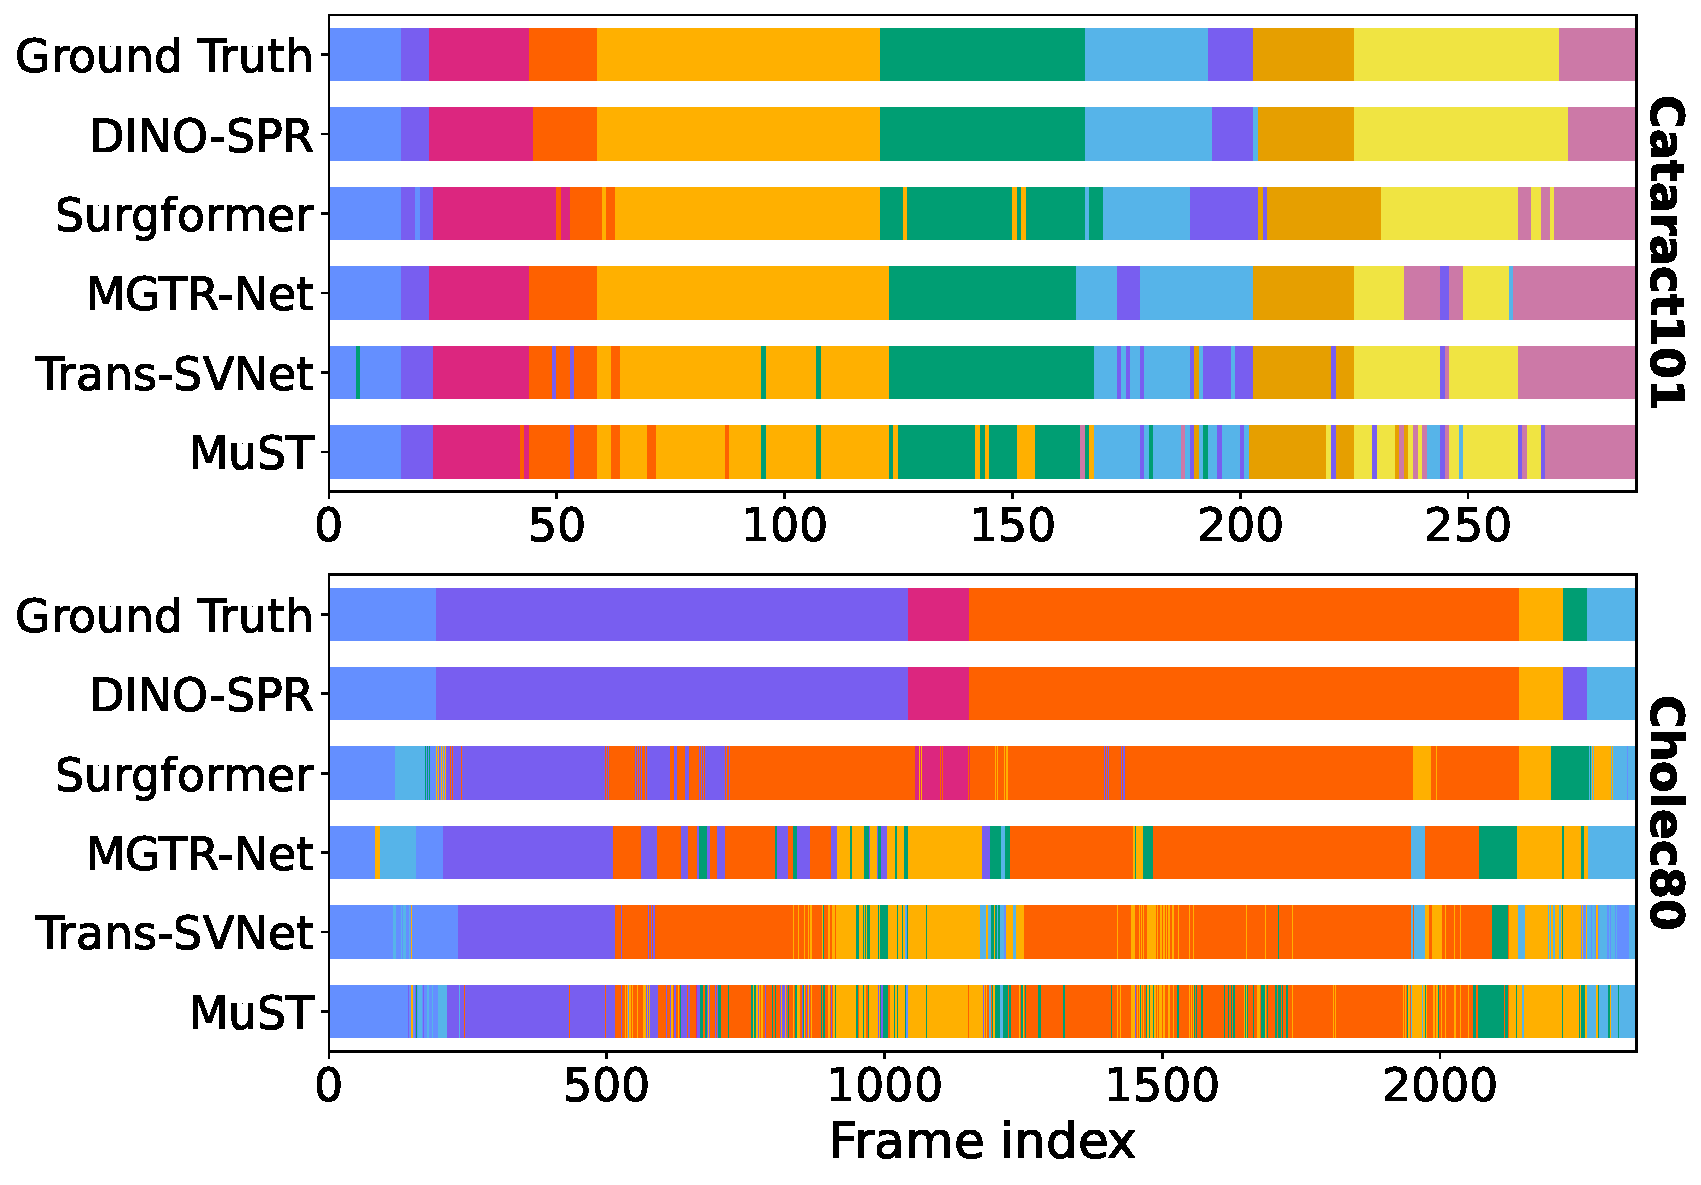
\includegraphics[width=\columnwidth]{resources/fig_phase_comparison_final_nolegend.pdf}
    \caption{Per-frame phase predictions of SPR-Teacher versus prior methods under the 6-shot setting on Cholec80 and Cataract101.}
    \label{fig:phase}
\end{figure}
\begin{figure*}[!ht]
    \centering
    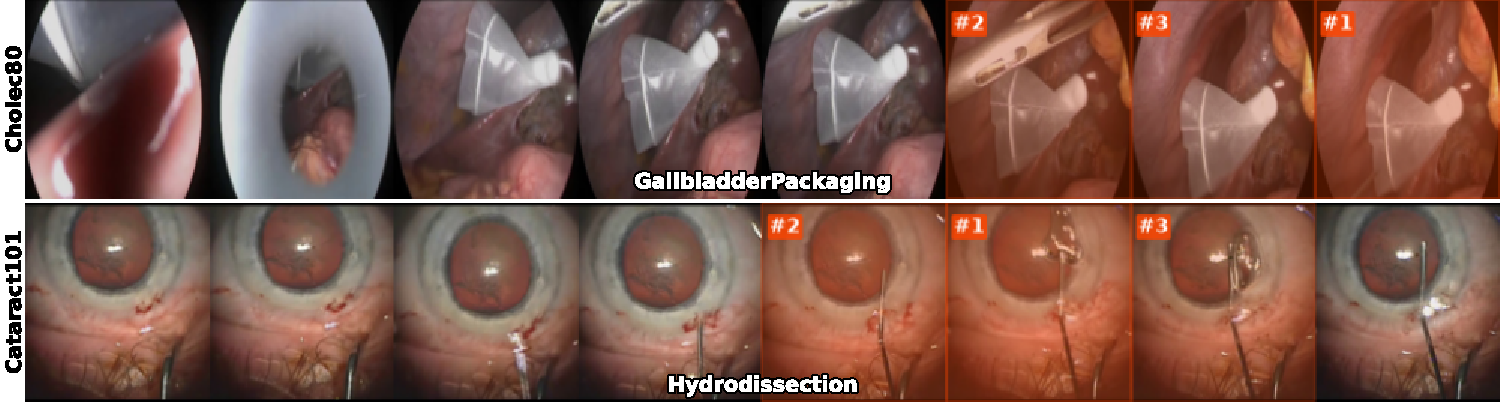
\includegraphics[width=\textwidth]{resources/temporal_final.pdf}
    \caption{Keyframe selection of the KPTF module. Within an 8-frame window, the top-3 frames with the largest temporal weights are highlighted (\#1--\#3); KPTF prioritizes frames with salient instrument-tissue interactions, which carry the strongest discriminative evidence.}
    \label{fig:keyframe}
\end{figure*}
\begin{figure}[!h]
    \centering
    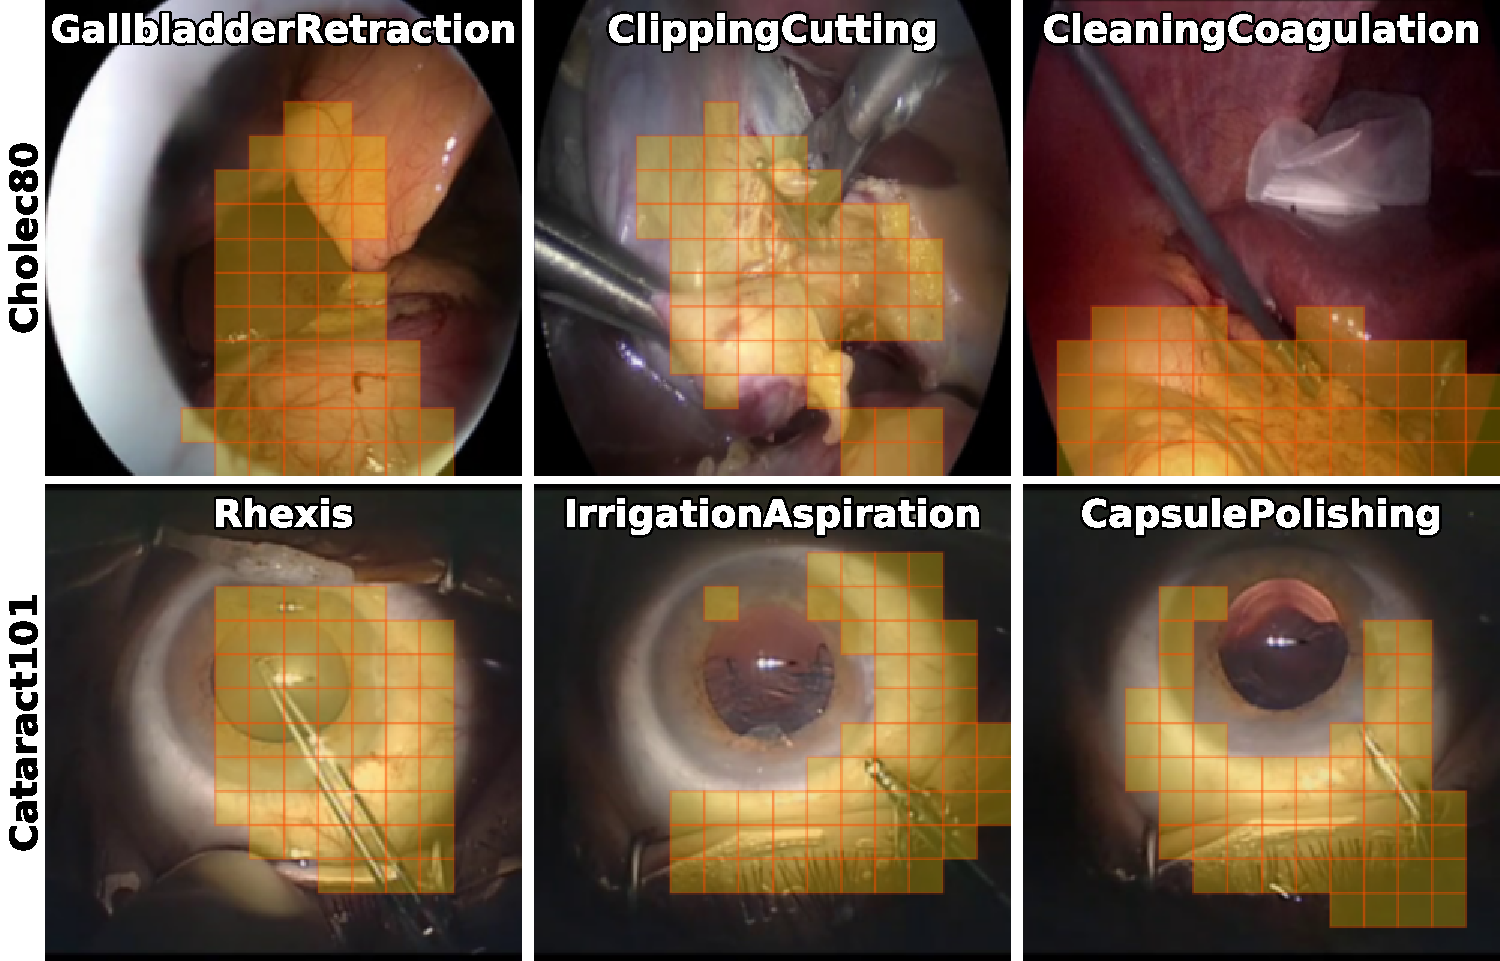
\includegraphics[width=\columnwidth]{resources/spatial_final.pdf}
    \caption{Spatial token selection of the SSTS module. Selected tokens (yellow) focus on instrument-tissue interactions while suppressing background, revealing the saliency prior guiding phase discrimination.}
    \label{fig:spatial}
\end{figure}


\subsection{Qualitative Analysis}
\subsubsection{Frame-level Phase Recognition}
% ref \label{fig:phase}：SPR 结果更准确，尤其 phase 边界切换、整体连续性、正确 phase 匹配。
Figure~\ref{fig:phase} compares per-frame predictions of DINO-SPR with prior
methods on test videos from Cholec80 and Cataract101.
DINO-SPR produces more continuous and accurate phase recognition, with cleaner boundaries
and far fewer fragmented predictions.
The improvement is most pronounced at phase transitions, where the spatiotemporal
module captures discriminative cues across frames to keep the prediction coherent,
while prior methods oscillate rapidly between adjacent phases.
Overall, the predicted sequences align closely with the ground-truth annotations,
showing that our end-to-end spatiotemporal design keeps accurate recognition even
under the limited supervision.
%
\subsubsection{Spatiotemporal Module Visualization}
% ref \label{fig:keyframe}：关键帧 KPTF weights top-3 highlight，展示 keyframe selection 有效性。
% ref \label{fig:spatial}：SSTS spatial token selection highlight，展示关注器械/组织区域而非背景。
Figure~\ref{fig:keyframe} visualizes the top-3 frames that KPTF selects within the input window.
The selected frames consistently capture informative moments such as
instrument-tissue interaction, while background-dominated views (e.g.,
out-of-focus or instrument-withdrawn scenes) receive low scores.
This shows that KPTF picks discriminative keyframes without explicit
supervision.
Figure~\ref{fig:spatial} visualizes the spatial token selection of SSTS, where
high-scoring patches concentrate on surgical instruments and tissue surfaces rather
than on irrelevant background.
These demonstrate that DINO-SPR focuses on the spatial and temporal
cues that carry the strongest discriminative evidence.




